  \item Usunięcie klienta \\
 
 Opis słowny - przypadek użycia procesowany w momencie, gdy użytkownik (klient)
 zdecyduje się zmienić swoje dane, na przykład na skutek zmiany miejsca
 zamieszkania, adresu e-mail itp. Dane powinny być zapisane w bazie danych
 natychmiast po wprowadzeniu ich przez użytkownika i wszelkie zamówienia już
 realizowane a także te, które zostaną złożone w przyszłości
 
 \begin{longtable}{|p{5cm}|p{7cm}|}
 	\hline
	\textbf{Aktor} & Pracownik, Klient \\
	\hline
	\textbf{Warunki początkowe} & Klient znajdujący się w systemie, Pracownik
	posiadający odpowiednie uprawnienia
	\\
	\hline
	\textbf{Opis przebiegu interakcji} & Znalezienie klienta do usunięcia z systemu
	przez pracownika, wpisanie powodu decyzji, obsługa niezrealizowanych zleceń,
	usunięcie z systemu
	\\
	\hline
	\textbf{Sytuacje wyjątkowe} & Brak
	\\
	\hline
	\textbf{Warunki końcowe} & Usunięcie klienta z systemu, zachowanie spójności
	bazy danych
	\\
	\hline
 \end{longtable}

\item Usunięcie klienta - scenariusz główny \\
  \begin{tabularx}{\linewidth}{ c X }
  Aktor: & Pracownik \\
  Opis: & Klienta można usunąć administracyjnie na przykład z powodów
  naruszenia regulaminu.\\
  \end{tabularx}
  \begin{enumerate}
    \item Pracownik sklepu wyszukuje klienta o konkretnym imieniu i nazwisku
    (lub według innych kryteriów)
    \item Pracownik wybiera opcję usunięcia klienta. 
    \item Pracownik wpisuje powód, dla którego usuwa użytkownika (informacja ta
    będzie przesłana do klienta w wiadomości e-mail)
    \item Pracownik wypełnia dane dotyczące kwestii niezrealizowanych zamówień i
    nieotrzymanych płatności
    \item Obie informacji (z poprzednich 2 kroków) są przekazywane na podany
    przez użytkownika adres e-mail
    \item Dane są przechowywane przez Okres Magazynowania Danych (patrz
    Wymagania Niefunkcjonalne punkt \ref{itm:OMD}) - w tym czasie użytkownik
    może złożyć reklamację i ewentualnie odzyskać dostęp do konta
    \item Po tym czasie, jeśli prośba o przywrócenie konta nie zostanie
    pozytywnie rozpatrzona, dane są na stałe usuwane z systemu
  \end{enumerate}
  
  
  \item Usunięcie klienta - scenariusz alternatywny - użytkownik składa
  pozytywnie zweryfikowaną reklamację
  \\
  \begin{tabularx}{\linewidth}{ c X }
  Aktor: & Pracownik \\
  Opis: & Klienta można usunąć administracyjnie na przykład z powodów
  naruszenia regulaminu.\\
  \end{tabularx}
  \begin{enumerate}
    \item Kroki 1-5 jak w scenariuszu głównym
    \item Użytkownik otrzymuje decyzję o zatrzymaniu procesu usuwania z systemu
    \item Klient decyduje, czy przywrócić stan zamówień sprzed rozpoczęcia
    procesowania przypadku użycia Usunięcie Klienta
    \item Klientowi zostają przydzielone wszystkie dane, jakie miał przed
    rozpoczęciem usuwania
  \end{enumerate}
  
  
  
  
  \begin{figure}[H]
    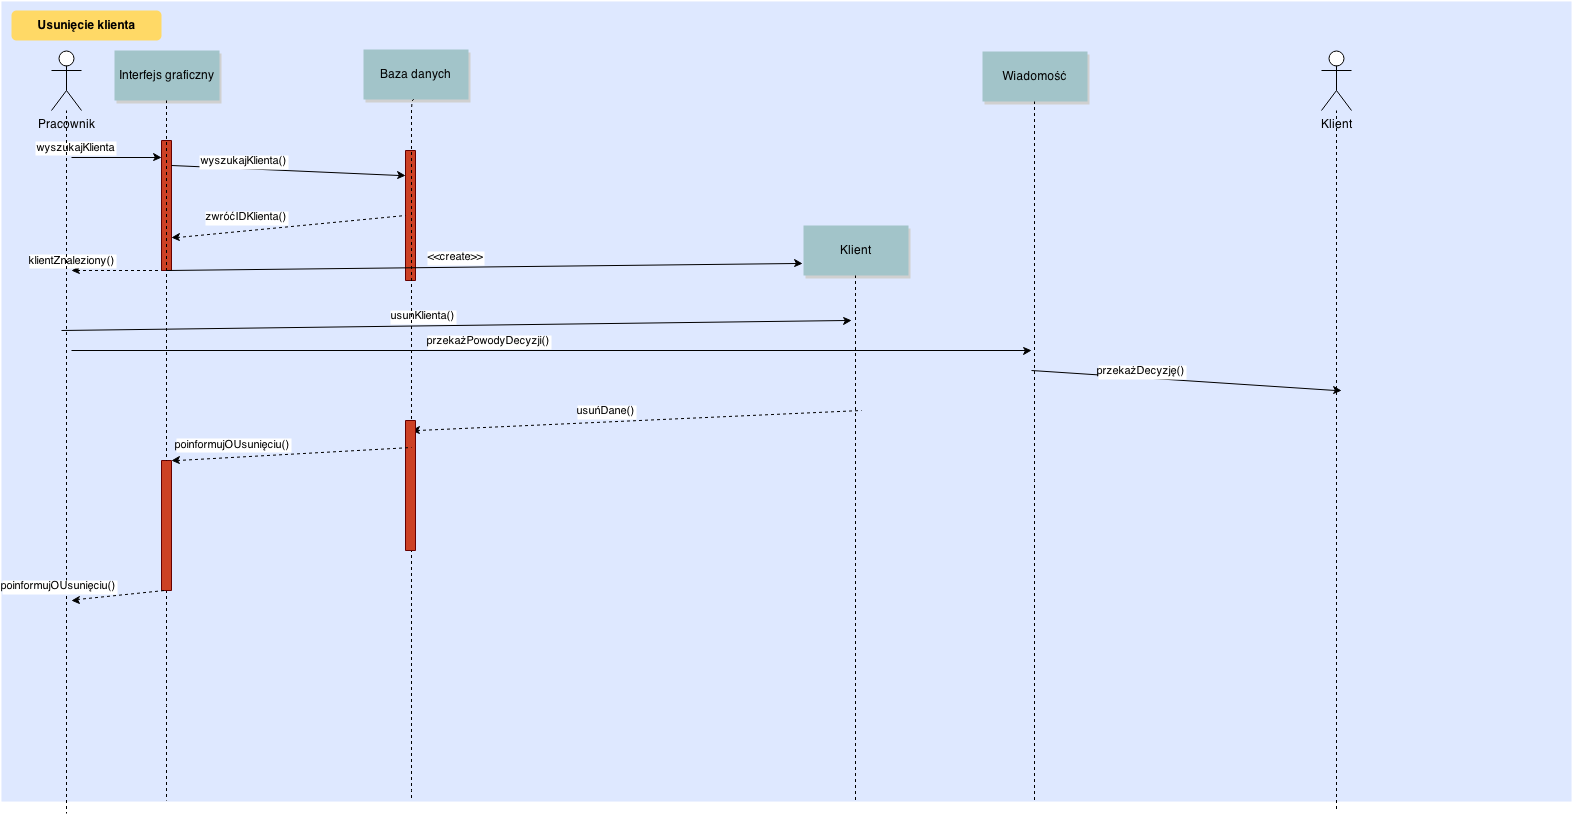
\includegraphics[width=\textwidth,
    height=0.5\textheight]{graphics/UseCase/Klient/UsuniecieKlientaSD.png}
  \caption{Diagram sekwencji dla przypadku użycia Usunięcie Klienta -
  scenariusz główny}
\end{figure}